\documentclass[12pt]{article}
\usepackage[margin=1in]{geometry}
\usepackage{amsmath,amsthm,amssymb}

% Ignore spaces in filenames
\usepackage[space]{grffile}

\usepackage[T1]{fontenc}
\usepackage{bigfoot} % to allow verbatim in footnote
\usepackage[numbered,framed]{matlab-prettifier}
\usepackage{filecontents}
\usepackage{graphicx}
\usepackage[normalem]{ulem}

\let\ph\mlplaceholder % shorter macro
\lstMakeShortInline"

\lstset{
  style              = Matlab-editor,
  basicstyle         = \mlttfamily,
  escapechar         = ",
  mlshowsectionrules = true,
}

\title{MAE 275 - Homework 5}
\author{John Karasinski}

\begin{document}
\maketitle

\section{Defining the System}
The lateral linearized aircraft equations of motion can be expressed in state space form, with state variables $\Delta v, \Delta p, \Delta r, \Delta \varphi, \Delta \psi $, as
\begin{equation*}
A =
\begin{bmatrix}
    Y_v & Y_p & \left[ Y_r-u_0 \right] & g\cos \theta_0 & 0 \\
    L_v^\prime & L_p^\prime & L_r^\prime & 0 & 0 \\
    N_v^\prime & N_p^\prime & N_r^\prime & 0 & 0 \\
    0 & 1 & \tan \theta_0 & 0 & 0 \\
    0 & 0 & \sec \theta_0 & 0 & 0
\end{bmatrix}\\
\end{equation*}

\noindent Relevant B, C, and D matrices can also be formed
\begin{equation*}
B =
\begin{bmatrix}
     Y_{\delta_r}       & Y_{\delta_a} \\ 
     L_{\delta_r}^\prime & L_{\delta_a}^\prime \\
     N_{\delta_r}^\prime & N_{\delta_a}^\prime \\
     0           & 0 \\
     0           & 0 \\
\end{bmatrix}
\end{equation*}

\begin{equation*}
C =
\begin{bmatrix}
    1/u_0 & 0 & 0 & 0 & 0\\
    0     & 0 & 1 & 0 & 0\\
    0     & 0 & 0 & 1 & 0\\
\end{bmatrix}
\end{equation*}

\begin{equation*}
D =
\begin{bmatrix}
     0 & 0 \\
     0 & 0 \\
     0 & 0 \\
\end{bmatrix}
\end{equation*}

\noindent with $x = [\Delta v, \Delta p, \Delta r, \Delta \varphi, \Delta \psi]$ and $u =[\Delta \delta_r, \Delta \delta_a]$.

\noindent Plugging in the data for the DC-8 aircraft in Flight Condition 8002 from Appendix A of "Aircraft Dynamics and Automatic Control" yields
\begin{equation*}
A =
\begin{bmatrix}
  -1.0080e-1 &          0 & -4.6820e+2 & +3.2200e+1  &          0 \\
  -5.7881e-3 & -1.2320e+0 & +3.9700e-1 &          0  &          0 \\
  +2.7787e-3 & -3.4600e-2 & -2.5700e-1 &          0  &          0 \\
           0 &          1 &          0 &          0  &          0 \\
           0 &          0 &          1 &          0  &          0 \\

\end{bmatrix}
\end{equation*}

\begin{equation*}
B =
\begin{bmatrix}
  +1.3480e+1 &          0 \\
  +3.9200e-1 & -1.6200e+0 \\
  -8.6400e-1 & -1.8750e-2 \\
           0 &          0 \\
           0 &          0 \\
\end{bmatrix}
\end{equation*}

\begin{equation*}
C =
\begin{bmatrix}
   +2.1358e-3 &           0 &           0  &          0 &           0 \\
            0 &           0 &           1  &          0 &           0 \\
            0 &           0 &           0  &          1 &           0 \\
\end{bmatrix}
\end{equation*}

\begin{equation*}
D =
\begin{bmatrix}
     0  &   0 \\
     0  &   0 \\
     0  &   0 \\
\end{bmatrix}
\end{equation*}


\clearpage
\section{Designing the Controller}

% The transfer function of the system, $VZ-4$, was identified as
% \begin{filecontents*}{code.m}
%             (s+1) (s+0.137)
%   -----------------------------------
%   (s+0.8223) (s^2 - 0.6401s + 0.5326)
% \end{filecontents*}
% \lstinputlisting[]{code.m}

Two controllers were designed. The first controller, $Gc_{\phi}$ was designed as
\begin{filecontents*}{code.m}
  -360.94 (s+1.413) (s+0.07616)
  -----------------------------
         s (s+100) (s+3)
\end{filecontents*}
\lstinputlisting[]{code.m}

\noindent This controller was determined using loop-shaping principles such that it had a roll-attitude bandwidth of $\sim$3 rad/sec (-3dB criterion) and a minimum overshoot in step response. \\

\noindent The second controller, $Gc_r$ was designed as
\begin{filecontents*}{code.m}
  21.969 (s-1.86)
  ----------------
  (s+10) (s+8.199)
\end{filecontents*}
\lstinputlisting[]{code.m}

\noindent This controller was determined using loop-shaping principles such that it had a bandwidth of $\sim$1 rad/sec (-3dB criterion), giving a factor of approximately three between r-loop and $\phi$-loop bandwidths. \\

\noindent Additionally, both controllers have:

more poles than zeros (are strictly proper compensators)

gain margins of at least 12dB

phase margins of at least 40 deg

 

% \begin{figure}[h]
% \begin{center}
% 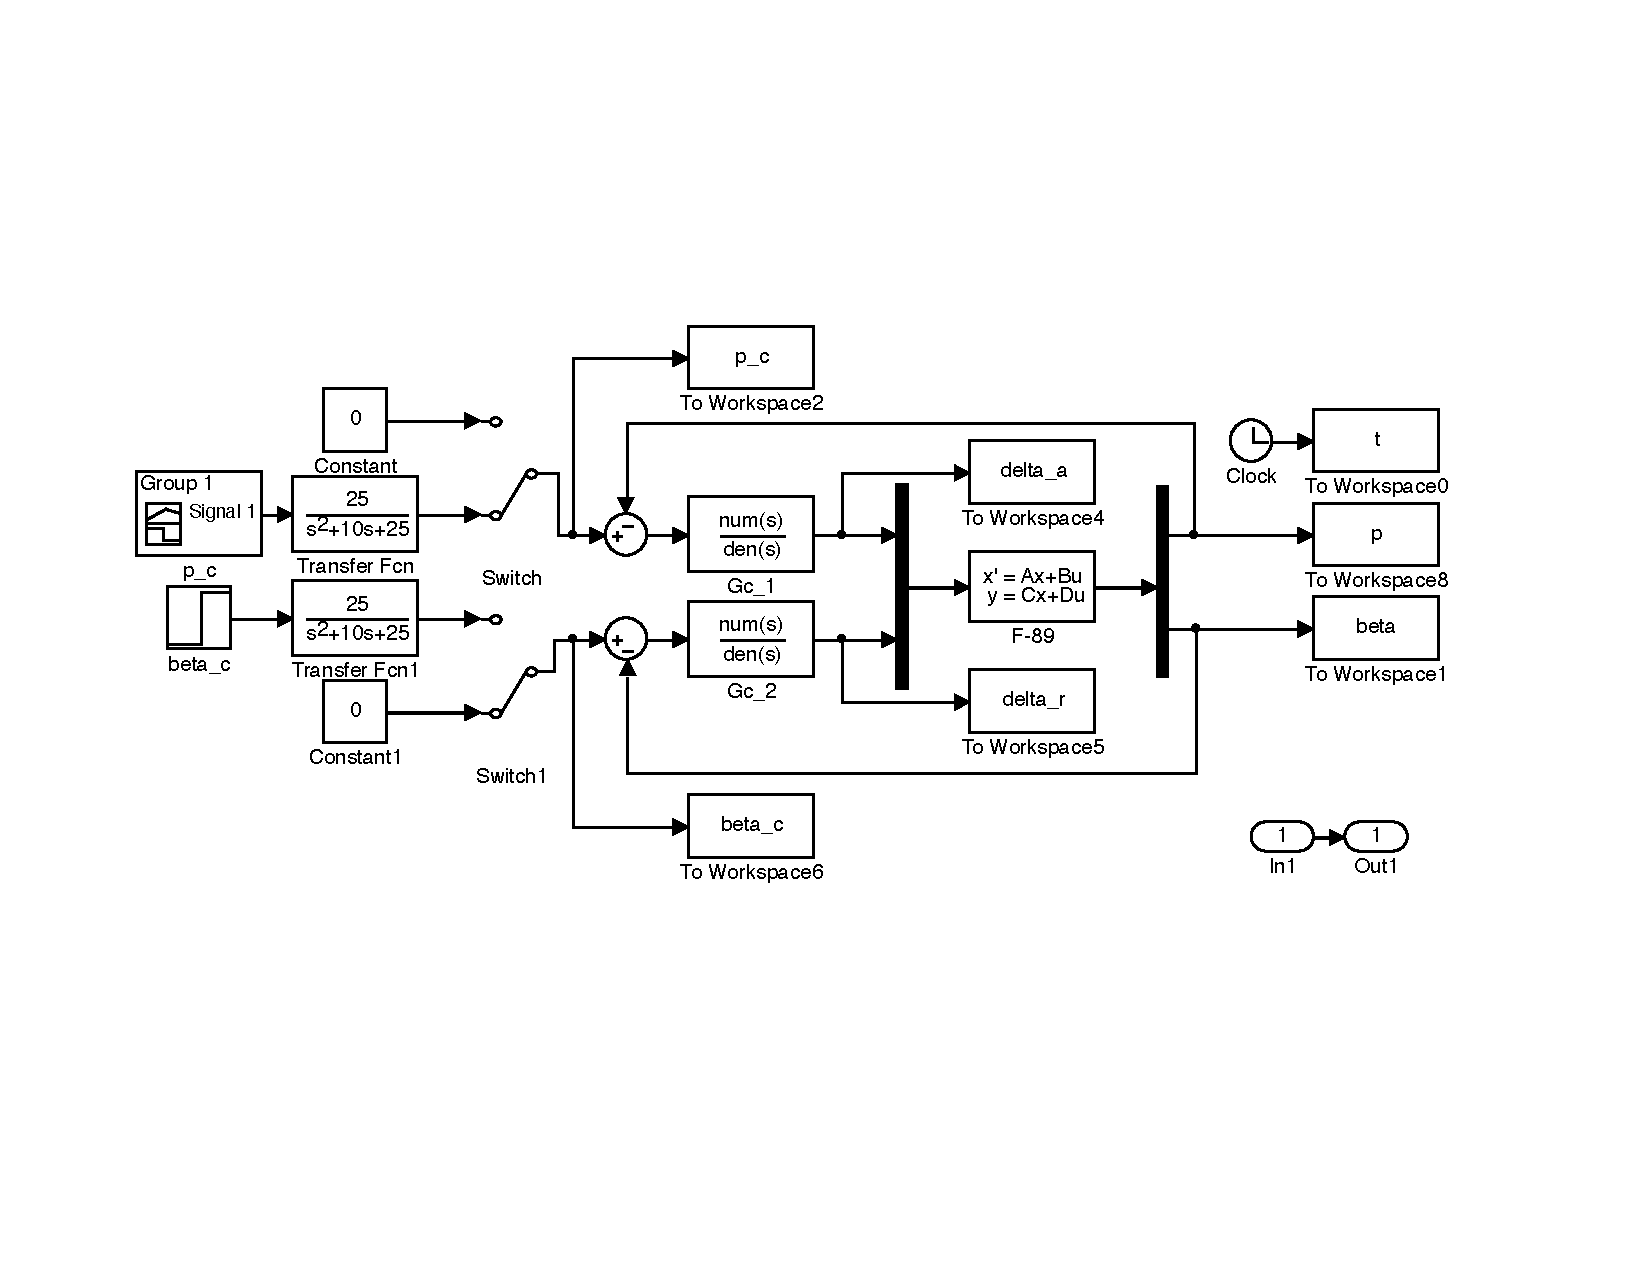
\includegraphics[width=.9\textwidth]{figures/simulink}
% \caption{Simulink Diagram}
% % \label{}
% \end{center}
% \end{figure}

\end{document}
